%%%%%%%%%%%%%%%%%%%%%%%%%%%%%%%%%%%%%%%%%%%%%%%%%%%%%%%%%%%%
%%  This Beamer template was created by Cameron Bracken.
%%  Anyone can freely use or modify it for any purpose
%%  without attribution.
%%
%%  Last Modified: January 9, 2009
%%

\documentclass[xcolor=x11names,compress]{beamer}

%% General document %%%%%%%%%%%%%%%%%%%%%%%%%%%%%%%%%%
\usepackage{graphicx}
\usepackage{tikz}
\usetikzlibrary{decorations.fractals}
%%%%%%%%%%%%%%%%%%%%%%%%%%%%%%%%%%%%%%%%%%%%%%%%%%%%%%


%% Beamer Layout %%%%%%%%%%%%%%%%%%%%%%%%%%%%%%%%%%
\useoutertheme[subsection=false,shadow]{miniframes}
\useinnertheme{default}
\usefonttheme{serif}
\usepackage{palatino}

\setbeamerfont{title like}{shape=\scshape}
\setbeamerfont{frametitle}{shape=\scshape}

\setbeamercolor*{lower separation line head}{bg=DeepSkyBlue4} 
\setbeamercolor*{normal text}{fg=black,bg=white} 
\setbeamercolor*{alerted text}{fg=red} 
\setbeamercolor*{example text}{fg=black} 
\setbeamercolor*{structure}{fg=black} 
 
\setbeamercolor*{palette tertiary}{fg=black,bg=black!10} 
\setbeamercolor*{palette quaternary}{fg=black,bg=black!10} 

\renewcommand{\(}{\begin{columns}}
\renewcommand{\)}{\end{columns}}
\newcommand{\<}[1]{\begin{column}{#1}}
\renewcommand{\>}{\end{column}}
%%%%%%%%%%%%%%%%%%%%%%%%%%%%%%%%%%%%%%%%%%%%%%%%%%




\begin{document}


%%%%%%%%%%%%%%%%%%%%%%%%%%%%%%%%%%%%%%%%%%%%%%%%%%%%%%
%%%%%%%%%%%%%%%%%%%%%%%%%%%%%%%%%%%%%%%%%%%%%%%%%%%%%%
\section{\scshape Why this DB?}
\begin{frame}
\title{BioBanks Catalog}
%\subtitle{SUBTITLE}
\author{
	Hocine Bendou\\
	{\it South African National Bioinformatics Institute}\\
}
\date{
	\begin{tikzpicture}[decoration=Koch curve type 2] 
		\draw[DeepSkyBlue4] decorate{ decorate{ decorate{ (0,0) -- (3,0) }}}; 
	\end{tikzpicture}  
	\\
	\vspace{1cm}
	\today
}
\titlepage
\end{frame}

%%%%%%%%%%%%%%%%%%%%%%%%%%%%%%%%%%%%%%%%%%%%%%%%%%%%%%
%%%%%%%%%%%%%%%%%%%%%%%%%%%%%%%%%%%%%%%%%%%%%%%%%%%%%%
%\begin{frame}{Introduction}
%\tableofcontents
%\end{frame}

%%%%%%%%%%%%%%%%%%%%%%%%%%%%%%%%%%%%%%%%%%%%%%%%%%%%%%
%%%%%%%%%%%%%%%%%%%%%%%%%%%%%%%%%%%%%%%%%%%%%%%%%%%%%%
\subsection{frame 1}
\begin{frame}{Problematic}
\begin{itemize}
\item Three biorepositories in three different Africa countries
\item Biorepositories: specialised stores for biospecimens
\item Different Laboratory Information Management System (LIMS) 
\item Access to LIMS is restricted from outside
\item Multiple queries/multiple access to search the biorepositories 
\end{itemize}
\end{frame}

%%%%%%%%%%%%%%%%%%%%%%%%%%%%%%%%%%%%%%%%%%%%%%%%%%%%%%
%%%%%%%%%%%%%%%%%%%%%%%%%%%%%%%%%%%%%%%%%%%%%%%%%%%%%%
\subsection{frame 2}
\begin{frame}{Solution proposed}

\begin{columns}[T]
 \begin{column}{.5\textwidth}
  \begin{block}{}
    \begin{itemize}
     \item Provide a unified platform for scientists
     \item Implement a custom database to house LIMS data
    \end{itemize}
  \end{block}
 \end{column}
 \begin{column}{.5\textwidth}
  \begin{block}{}
   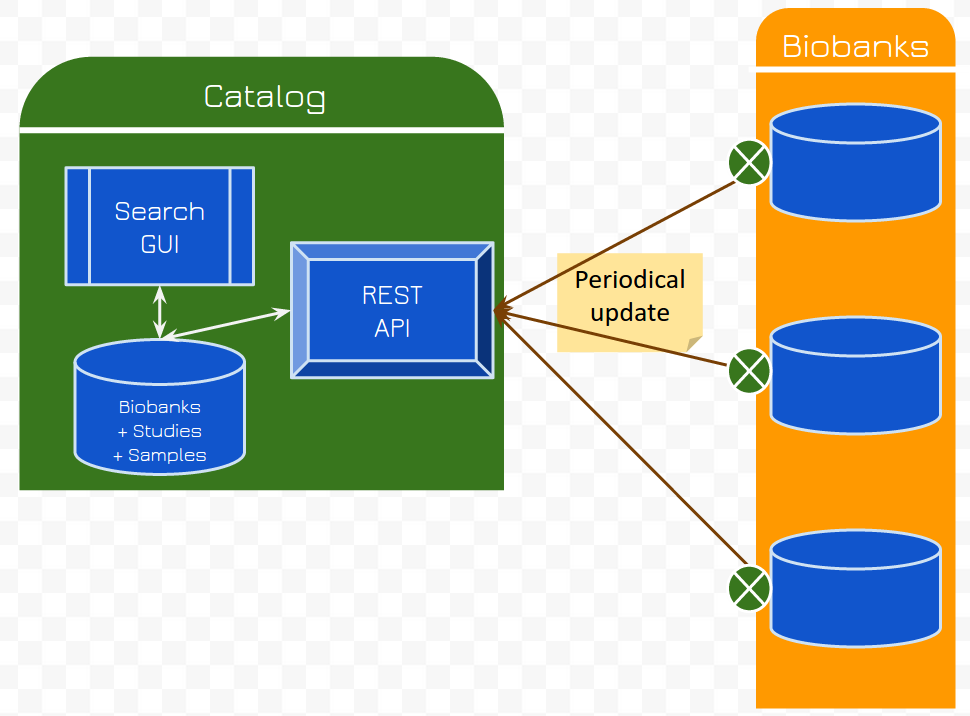
\includegraphics[width=6cm, height=5cm]{images/solution.png}
  \end{block}
 \end{column}
\end{columns}


\end{frame}

%%%%%%%%%%%%%%%%%%%%%%%%%%%%%%%%%%%%%%%%%%%%%%%%%%%%%%
%%%%%%%%%%%%%%%%%%%%%%%%%%%%%%%%%%%%%%%%%%%%%%%%%%%%%%
\section{\scshape Type of data}
\subsection{frame 1}
\begin{frame}{ER Diagram}
  \begin{block}{}
   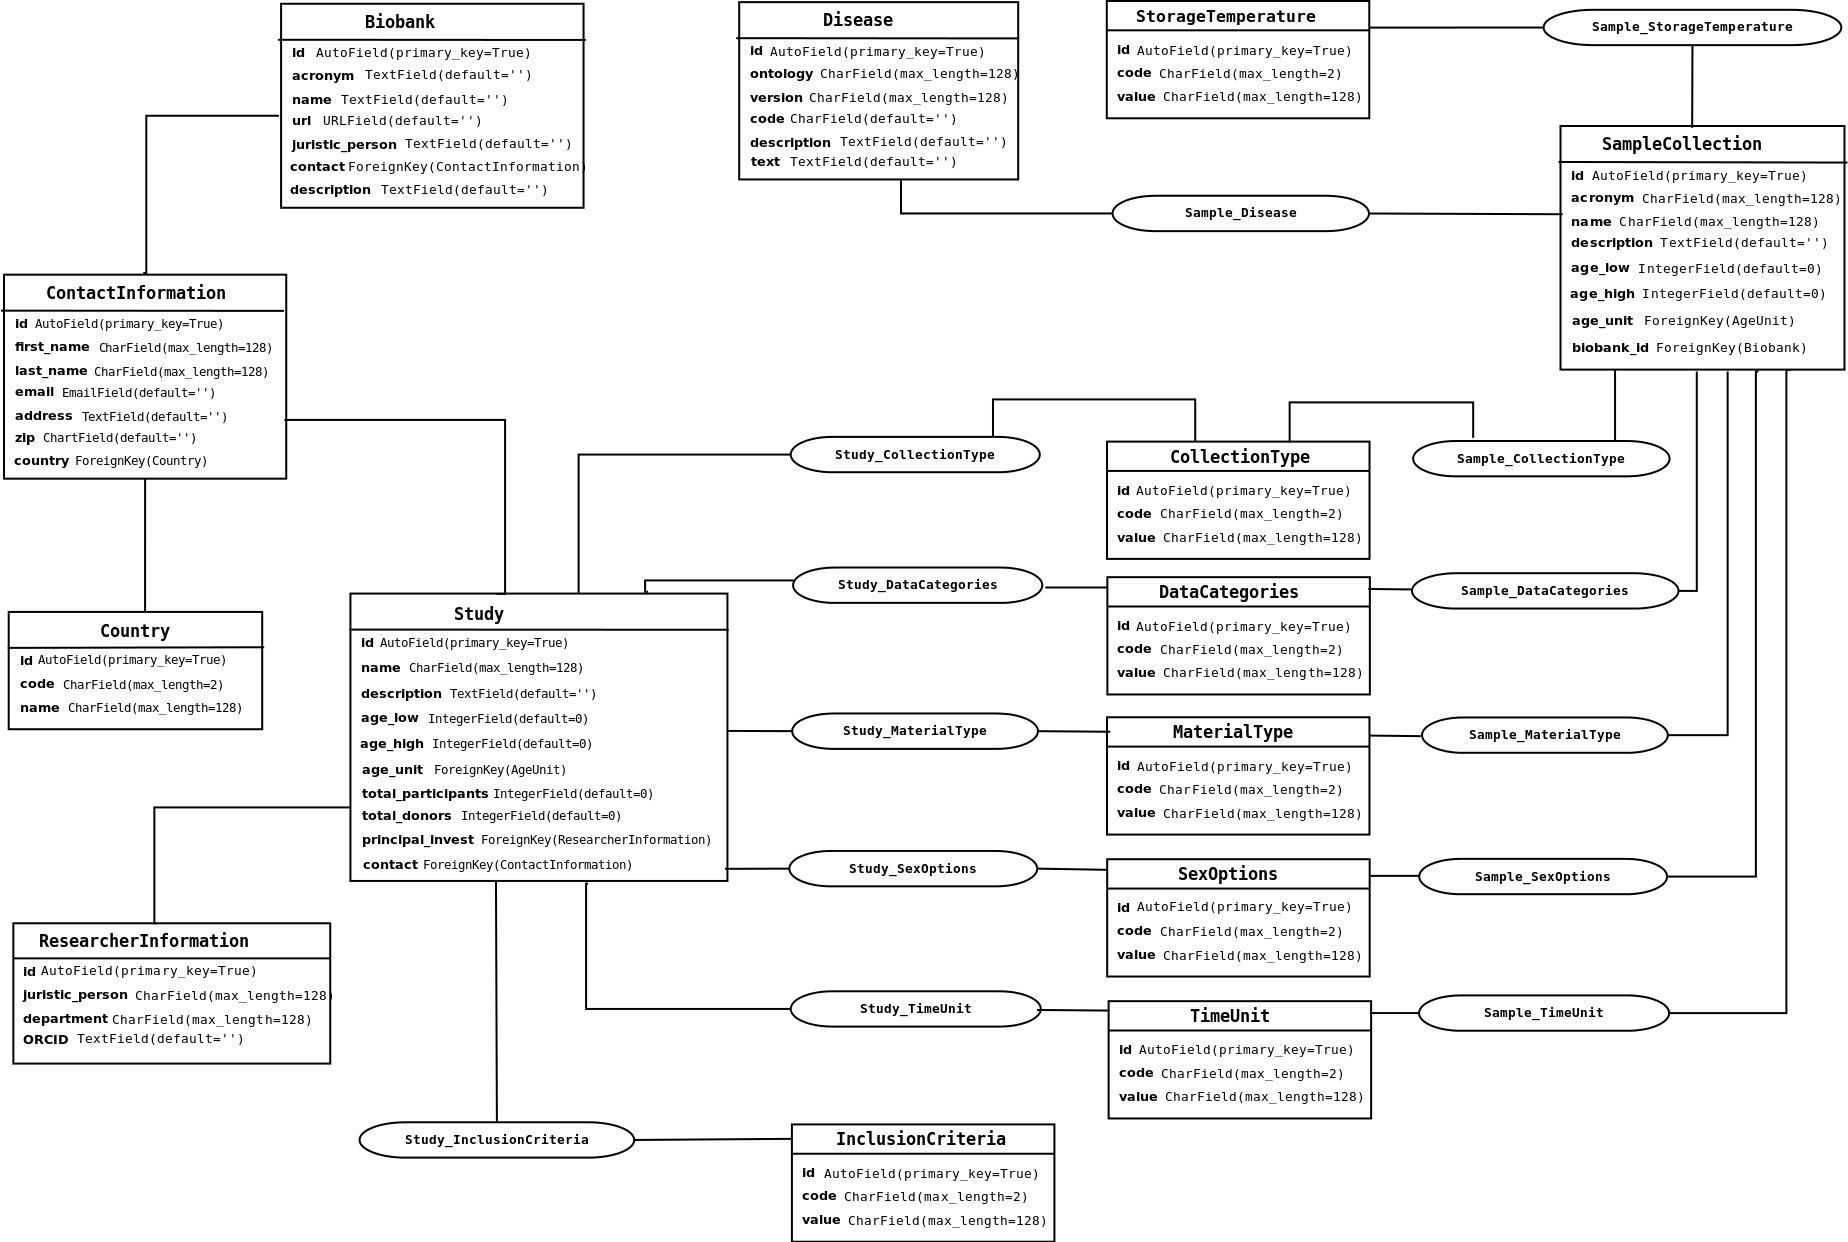
\includegraphics[width=11cm, height=7cm]{images/ER_Diagram.png}
  \end{block}
\end{frame}

%%%%%%%%%%%%%%%%%%%%%%%%%%%%%%%%%%%%%%%%%%%%%%%%%%%%%%
%%%%%%%%%%%%%%%%%%%%%%%%%%%%%%%%%%%%%%%%%%%%%%%%%%%%%%
\section{\scshape Django}
\subsection{frame 1}
\begin{frame}{ER to database}
 \begin{columns}[T]
 \begin{column}{.5\textwidth}
  \begin{block}{}
    \begin{itemize}
     \item Database management system: SQLite, MySQL, etc.
     \item Structured query language
     \item Framework tools: Django, Flask, Pyramid, etc.
    \end{itemize}
  \end{block}
 \end{column}
 \begin{column}{.5\textwidth}
  \begin{block}{}
   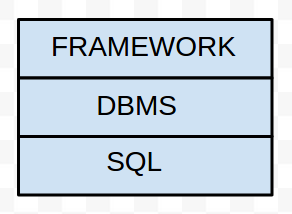
\includegraphics[width=4cm, height=4cm]{images/layers.png}
  \end{block}
 \end{column}
\end{columns}

\end{frame}

%%%%%%%%%%%%%%%%%%%%%%%%%%%%%%%%%%%%%%%%%%%%%%%%%%%%%%
%%%%%%%%%%%%%%%%%%%%%%%%%%%%%%%%%%%%%%%%%%%%%%%%%%%%%%
\subsection{frame 2}
\begin{frame}{Django}

\begin{columns}[T]
 \begin{column}{.6\textwidth}
  \begin{block}{}
    \begin{itemize}
     \item Free and open source web application framework, written in Python
     \item Develop dynamic websites faster and easier
     \item Support many different database servers, SQLite, PostgreSQL, etc.
    \end{itemize}
  \end{block}
 \end{column}
 \begin{column}{.4\textwidth}
  \begin{block}{}
   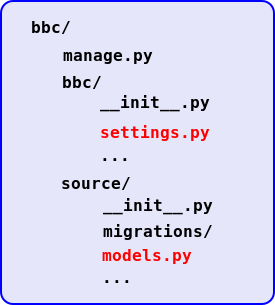
\includegraphics[width=4cm, height=3cm]{images/structure1.png}
  \end{block}
 \end{column}
\end{columns}

\end{frame}

%%%%%%%%%%%%%%%%%%%%%%%%%%%%%%%%%%%%%%%%%%%%%%%%%%%%%%
%%%%%%%%%%%%%%%%%%%%%%%%%%%%%%%%%%%%%%%%%%%%%%%%%%%%%%
\subsection{frame 3}
\begin{frame}{settings.py}
  \begin{block}{}
   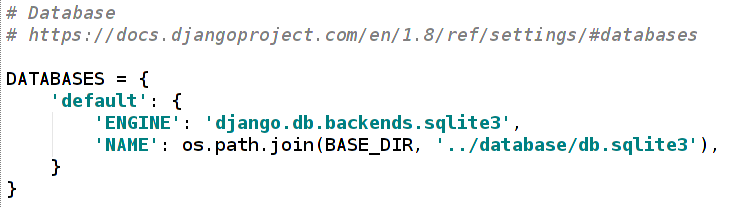
\includegraphics[width=7cm, height=4cm]{images/dbsettings.png}
  \end{block}
\end{frame}

%%%%%%%%%%%%%%%%%%%%%%%%%%%%%%%%%%%%%%%%%%%%%%%%%%%%%%
%%%%%%%%%%%%%%%%%%%%%%%%%%%%%%%%%%%%%%%%%%%%%%%%%%%%%%
\subsection{frame 4}
\begin{frame}{models.py}

\begin{columns}[T]
 \begin{column}{.6\textwidth}
  \begin{block}{}
    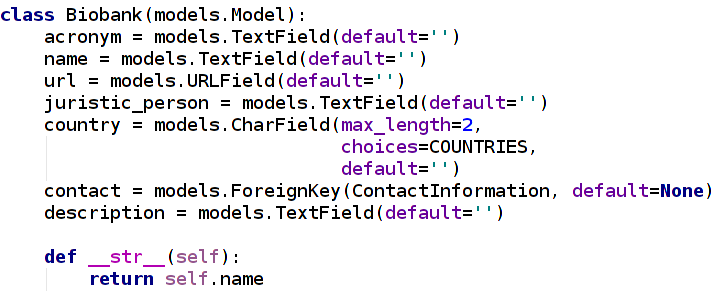
\includegraphics[width=6cm, height=4cm]{images/biobank.png}
  \end{block}
 \end{column}
 \begin{column}{.4\textwidth}
  \begin{block}{}
   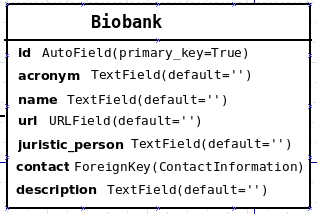
\includegraphics[width=3cm, height=3cm]{images/erbiobank.png}
  \end{block}
 \end{column}
\end{columns}

\end{frame}

%%%%%%%%%%%%%%%%%%%%%%%%%%%%%%%%%%%%%%%%%%%%%%%%%%%%%%
%%%%%%%%%%%%%%%%%%%%%%%%%%%%%%%%%%%%%%%%%%%%%%%%%%%%%%
\subsection{frame 5}
\begin{frame}{Database generation}

\begin{columns}[T]
 \begin{column}{.5\textwidth}
  \begin{block}{}
    
\includegraphics[width=5cm, height=1cm]{images/command1.png}
  \end{block}
  \begin{block}{}
    
\includegraphics[width=5cm, height=1cm]{images/command2.png}
  \end{block}
 \end{column}
 \begin{column}{.5\textwidth}
  \begin{block}{}
   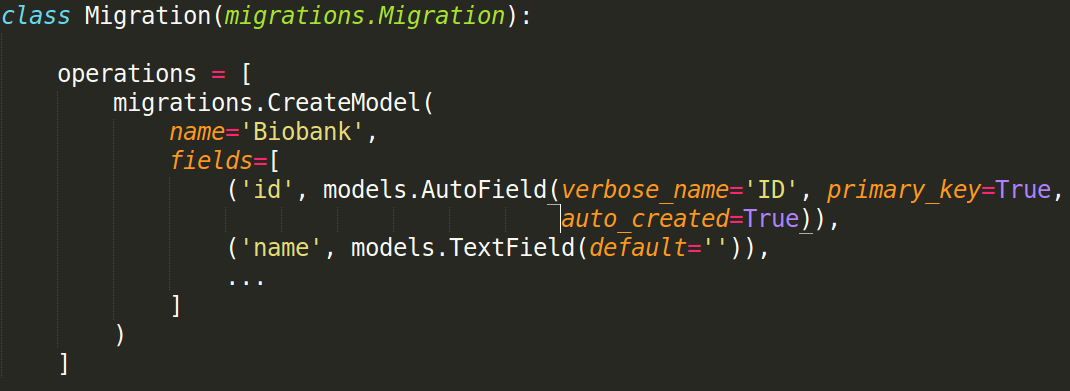
\includegraphics[width=5.5cm, height=4.5cm]{images/migrations.png}
  \end{block}
 \end{column}
\end{columns}

\end{frame}


%%%%%%%%%%%%%%%%%%%%%%%%%%%%%%%%%%%%%%%%%%%%%%%%%%%%%%
%%%%%%%%%%%%%%%%%%%%%%%%%%%%%%%%%%%%%%%%%%%%%%%%%%%%%%
\section{\scshape Insert?}
\subsection{frame 1}
\begin{frame}{Add data}
  \begin{block}{}
    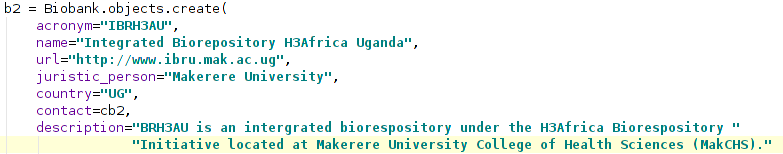
\includegraphics[width=11cm, height=5cm]{images/filldata.png}
  \end{block}
\end{frame}

%%%%%%%%%%%%%%%%%%%%%%%%%%%%%%%%%%%%%%%%%%%%%%%%%%%%%%
%%%%%%%%%%%%%%%%%%%%%%%%%%%%%%%%%%%%%%%%%%%%%%%%%%%%%%
\section{\scshape Select?}
\subsection{Frame 1}
\begin{frame}{Query data}
  \begin{block}{}
    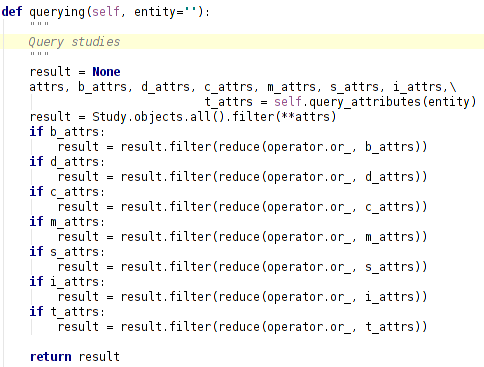
\includegraphics[width=10cm, height=5cm]{images/querying.png}
  \end{block}
\end{frame}

%%%%%%%%%%%%%%%%%%%%%%%%%%%%%%%%%%%%%%%%%%%%%%%%%%%%%%
%%%%%%%%%%%%%%%%%%%%%%%%%%%%%%%%%%%%%%%%%%%%%%%%%%%%%%
\subsection{Frame 2}
\begin{frame}{}
  \begin{block}{}
    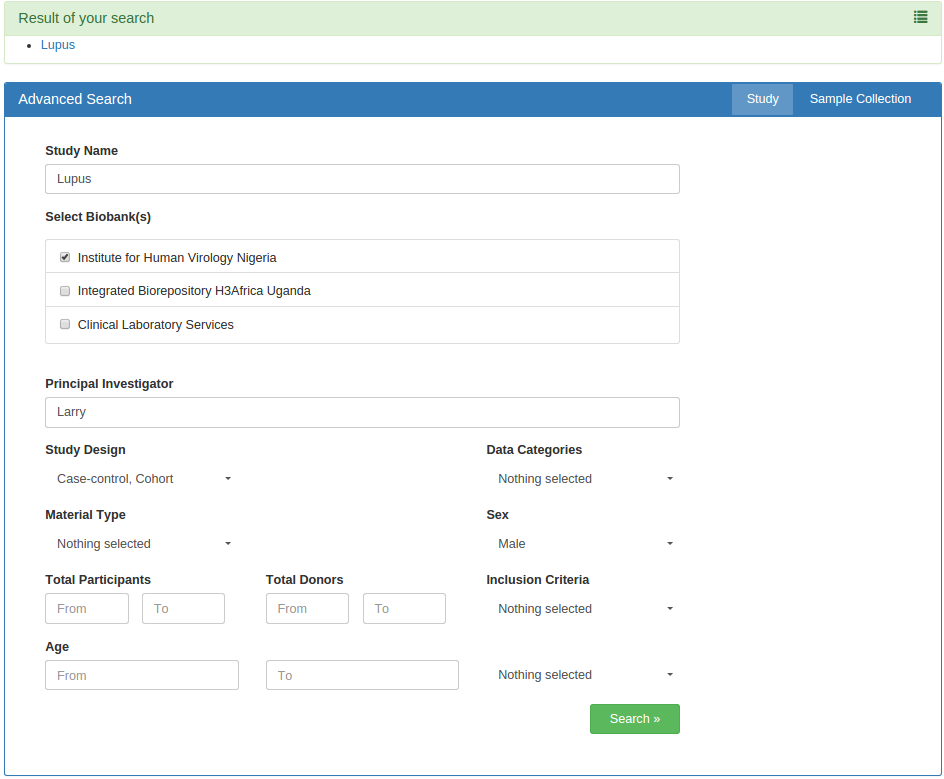
\includegraphics[width=9cm, height=6cm]{images/form.png}
  \end{block}
\end{frame}

%%%%%%%%%%%%%%%%%%%%%%%%%%%%%%%%%%%%%%%%%%%%%%%%%%%%%%
%%%%%%%%%%%%%%%%%%%%%%%%%%%%%%%%%%%%%%%%%%%%%%%%%%%%%%
\section{\scshape Pros \& cons}
\subsection{Frame 1}
\begin{frame}{}
  \begin{itemize}
   \item \textbf{Pros:} Easy, less coding, faster(objects in RAM)
  \end{itemize}
  \begin{block}{}
    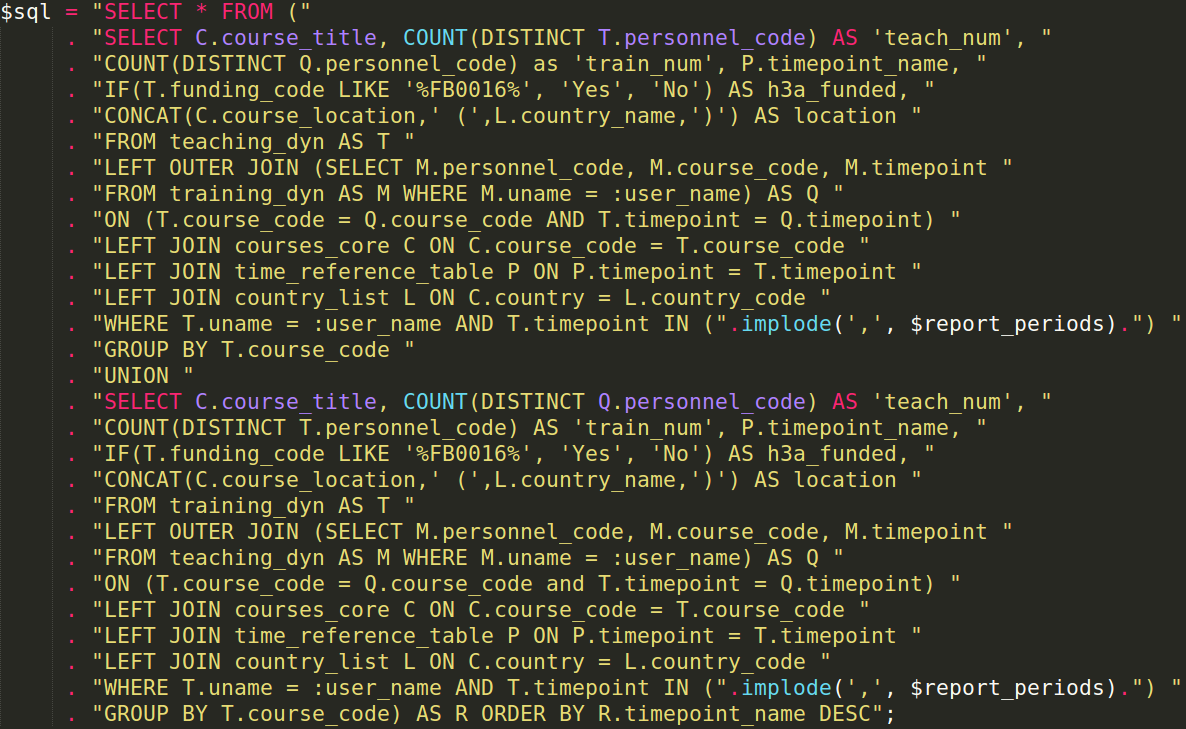
\includegraphics[width=10cm, height=6cm]{images/sql.png}
  \end{block}
  \begin{itemize}
   \item \textbf{Cons:} Many queries $\longrightarrow$ many objects $\longrightarrow$ less RAM
  \end{itemize}
\end{frame}

%%%%%%%%%%%%%%%%%%%%%%%%%%%%%%%%%%%%%%%%%%%%%%%%%%%%%%
%%%%%%%%%%%%%%%%%%%%%%%%%%%%%%%%%%%%%%%%%%%%%%%%%%%%%%
\subsection{Frame 2}
\begin{frame}{Conclusion}
\begin{columns}[T]
 \begin{column}{.5\textwidth}
  \begin{block}{}
    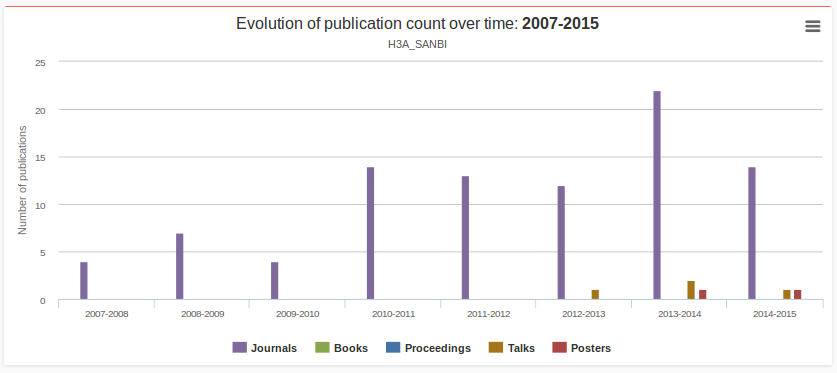
\includegraphics[width=5cm, height=4cm]{images/graphic.png}
  \end{block}
 \end{column}
 \begin{column}{.5\textwidth}
  \begin{block}{}
   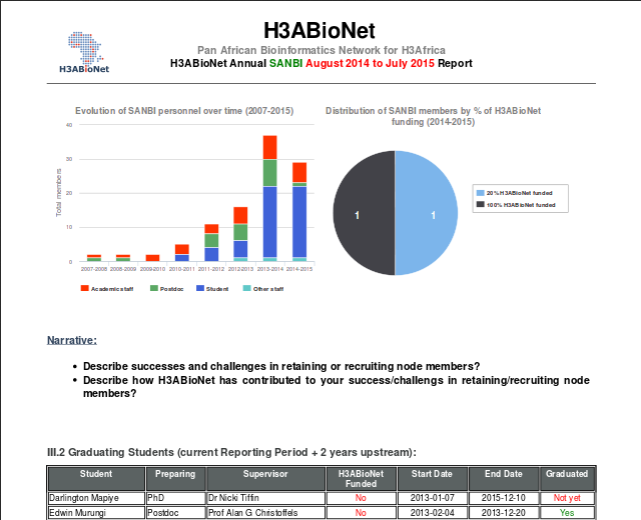
\includegraphics[width=5cm, height=6cm]{images/report.png}
  \end{block}
 \end{column}
\end{columns}
\end{frame}

\end{document}